\chapter{Results}
In the next section two error metrics are briefly described, followed by evaluations of each experiment. At the beginning of each section a small description of the problem setting is given, followed by the results and discussion.

\section{Error Metrics}
\label{Emetrics}
For this thesis two error metrics were considered:
\begin{itemize}
  \item \textbf{Point Distance:} Given two meshes with equal topology, meaning both meshes have the same amount of vertices and layout, the error computed is based on the distance between corresponding points. In general, the mean distance is computed over all point correspondences.
  \item \textbf{Face orientations:} The idea behind this method is based on the $\mathbf{Q}$ matrix mentioned in section \ref{faceDeform}. Given two topologically equal meshes, the $\mathbf{Q}$ matrix is computed for all corresponding faces. As it is of interest to investigate the difference in breast shapes, this error tries to quantify the variation of the $\mathbf{Q}$ matrices.
\end{itemize}

One drawback of the point distance method occurs when the two meshes are not aligned properly. This can be solved by applying the same algorithm mentioned in section \ref{align} before computing the error. One advantage of this method is the unit of the error, as it could be converted into a unit of distance, given the distance between two point is known in real world lengths. This error can also be computed when two meshes are not topologically equal by first finding the correspondences between vertices.\\
One advantage of the face orientation method is the invariance of translation and global rotation. This means that moving or rotating the mesh doesn't affect the error. On the other hand, the values of this error don't have a real world meaning and it is a lot harder to apply this method to topologically different meshes, as finding correspondences between faces is a lot more challenging.\\
The methods are depicted in figure \ref{fig:errordiag}. Both methods have their advantages and disadvantages, but due to the fact that alignment isn't a problem, the error metric used in this thesis is the point distance method.

\begin{figure}
\centering
\begin{subfigure}{.5\textwidth}
  \centering
  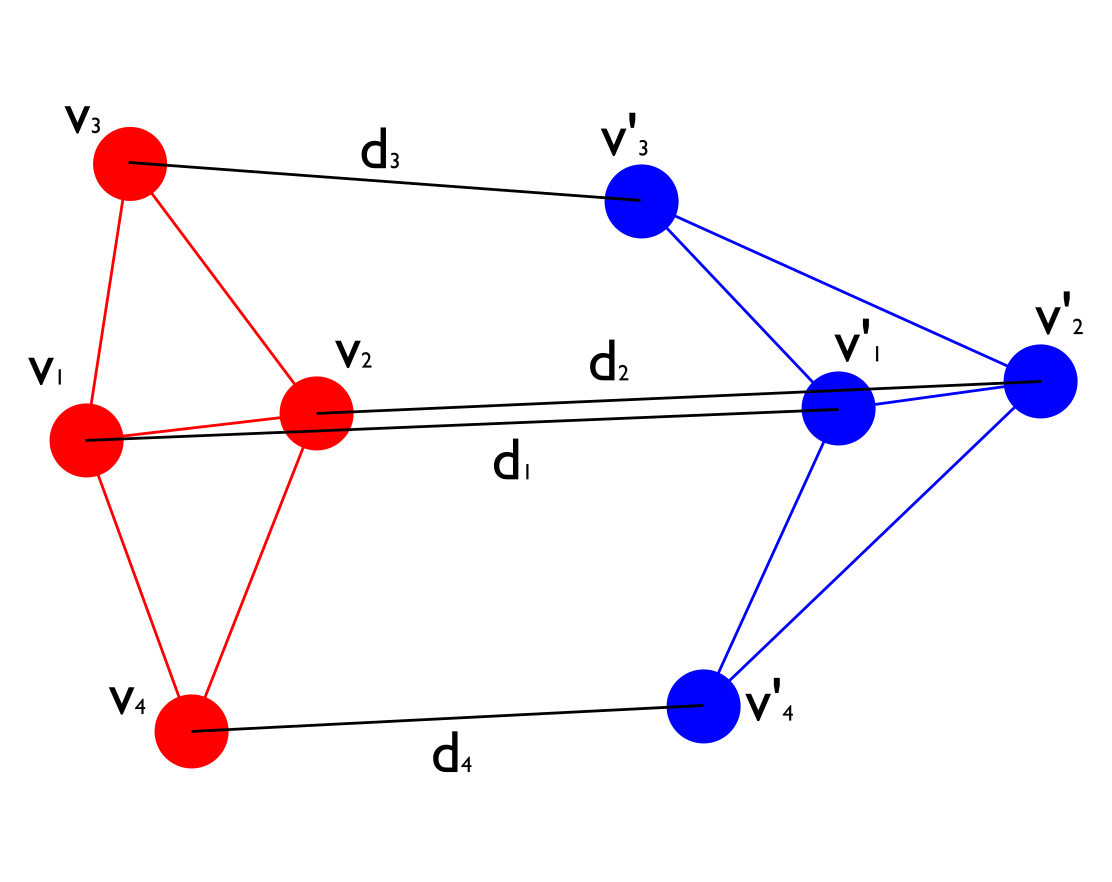
\includegraphics[width=.75\linewidth]{figures/pediag}
\end{subfigure}%
\begin{subfigure}{.5\textwidth}
  \centering
  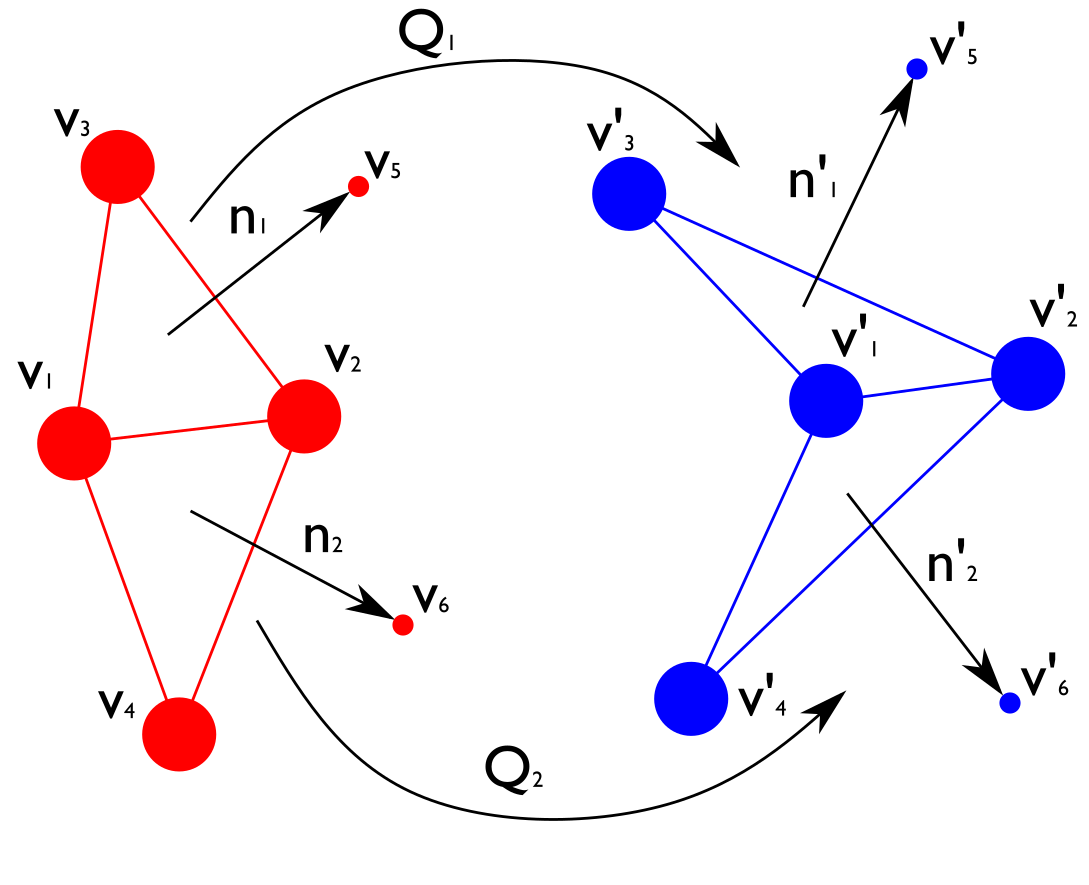
\includegraphics[width=.75\linewidth]{figures/dediag}
\end{subfigure}
\caption{The left image depicts distances between corresponding points of the mesh. The right image shows a representation of the information used to compute the $\mathbf{Q}$ matrix.}
\label{fig:errordiag}
\end{figure}

\section{Evaluation}
In the following section the evaluation methods, that were used, are explained. Optimally, when evaluating a prediction some representation of the true outcome, often called the "ground truth", is given. This is useful to quantify how acurate the prediction was.
\subsection{Mesh Point Error} % Compare to GT
For this method the comparison is done as explained in section \ref{Emetrics}. Before evaluating the point distances between a prediction and the ground truth, the meshes are aligned as mentioned in section \ref{align}. Additionally, the mean point distance error is computed by diving by the number of vertices in the mesh and also by diving by the diagonal of the largest bounding box over all examples to scale the error to a meaningful unit. Given a prediction of a mesh $M^{(p)}$ and the ground truth $M^{(g)}$ the problem can be stated as:
\begin{gather}
error = \frac{1}{nd_{max}}\sum_{i=1}^{n} \sqrt{\sum_{j=1}^3(M_{i,j}^{(p)} - M_{i,j}^{(g)})^2}
\end{gather}
where $n$ is the number of vertices of the mesh, $d_{max}$ is the diagonal length of the largest bounding box over all examples and the final result is a scalar value.
\subsection{Error Heat Map} % Compare to NRICP vs Ceres
The idea of this method is to generate a visualization of the error, indicating where the prediction failed to represent the ground truth the most. This can be accomplished by computing the error described in section \ref{Emetrics} but instead of adding up the errors keeping them separate for each vertex. This error per vertex is accumulated over multiple samples. Given the  k-th prediction of a mesh $M^{(p_k)}$ and the corresponding ground truth $M^{(g_k)}$ the problem can be described as:
\begin{gather}
e'_{i} = \sum_{k=1}^{m} \sqrt{\sum_{j=1}^3(M_{i,j}^{(p_k)} - M_{i,j}^{(g_k)})^2} \  \forall i=1 \dots n \text{ with } e = \frac{e'}{max(e'_{i}))}
\end{gather}

\section{Input Data for PCA}

\section{Learning Mapping}

\section{Parametric Models}
Given two parametric models and a test set of point clouds, both models process the point clouds as described in section \ref{fitModel}.


\chapter{Conclusion and Outlook}
